\documentclass{article}

\usepackage[most]{tcolorbox}
\usepackage{physics}
\usepackage{graphicx}
\usepackage{float}
\usepackage{amsmath}
\usepackage{amssymb}


\usepackage[utf8]{inputenc}
\usepackage[a4paper, margin=1in]{geometry} % Controla los márgenes
\usepackage{titling}

\title{Clase Agujeros Negros Cuánticos}
\author{Manuel Garcia.}
\date{\today}

\renewcommand{\maketitlehooka}{%
  \centering
  \vspace*{0.05cm} % Espacio vertical antes del título
}

\renewcommand{\maketitlehookd}{%
  \vspace*{2cm} % Espacio vertical después de la fecha
}

\newcommand{\caja}[3]{%
  \begin{tcolorbox}[colback=#1!5!white,colframe=#1!25!black,title=#2]
    #3
  \end{tcolorbox}%
}

\begin{document}
\maketitle

\section{}
\begin{figure}[H]
  \begin{center}
    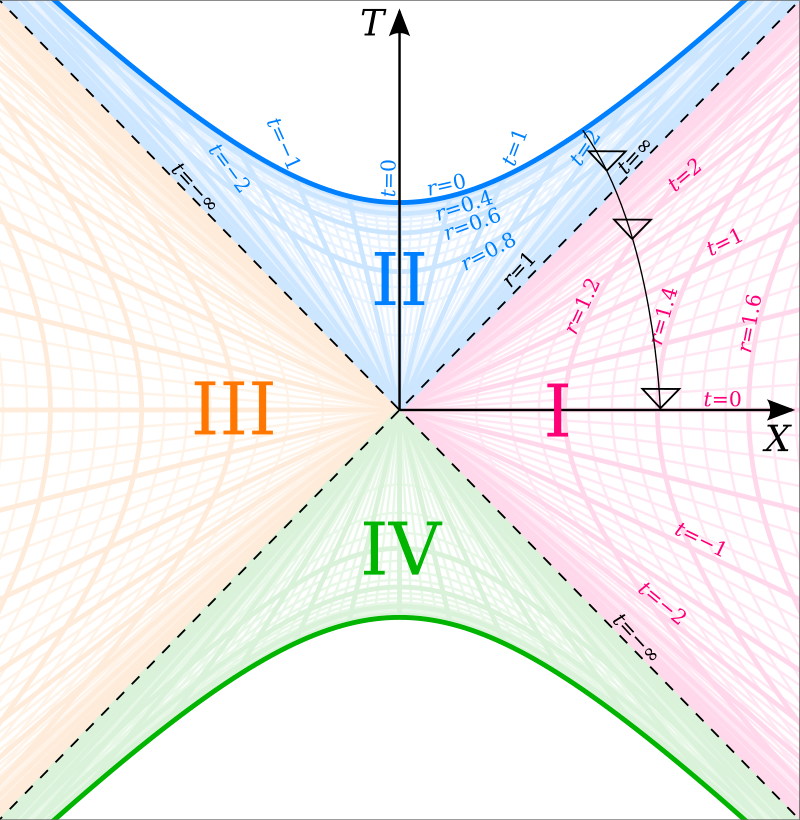
\includegraphics[width=0.35\textwidth]{kruskal.png}
  \end{center}
\end{figure}


De la clase anterior teníamos la ecuación de Klein-Gordon y sus soluciones 
\begin{gather*}
  (\Box - m^2 ) \phi = 0 \\
  \{\phi_\Omega ^ {(t) }(x) \} \qquad \qquad \phi_\Omega ^ {(t)}(x) = \phi _\Omega (t,x) \Theta_\epsilon(x) \\
  \Theta_\epsilon(x) := \frac{1}{2}\{\Theta(-\epsilon U) + \Theta(\epsilon V  )\} \qquad \qquad \text{Con }\epsilon = \pm 1  \\
  \phi_\Omega(t,\vec x) = \phi_\Omega (r) Y _{lm } (\theta,\phi) \frac{1}{\sqrt{2 \left|\omega\right|} } e ^ {- i \omega t }
\end{gather*}
Reemplazando $ \phi_\Omega (t,\vec x)  $ en la ecuación de Klein-Gordon 
\begin{gather*}
  \frac{1}{r^2 } \frac{d  }{d r } \left(r^2 f\left(r\right) \frac{d \phi_\Omega(r)  }{d r }\right) + \left(\frac{\omega^2 }{f(r) } - \frac{l(l+1) }{r^2 } - m^2 \right)\phi_\Omega(r) = 0  
\end{gather*}
Tenemos que la métrica $ ds^2 = g _{00 }  dt^2 + g _{ab }  dx^a dx^b  $ donde $ g _{00 } = - f(r)  $\\ 
\\
Sea la definición 
\begin{gather*}
  dr_* \equiv \frac{dr }{f(r) } \qquad   \rightarrow \qquad r_* = \displaystyle\int_{}^{} f^{-1} (r) dr \qquad\rightarrow \qquad\frac{d \hat f  }{d r_* } = \frac{d \hat f  }{f ^ {-1 }(r) dr}
\end{gather*}
Obteniendo 
\begin{gather*}
  \frac{d  }{d r_* } = f(r) \frac{d  }{d r } 
\end{gather*}
Lo cual podemos reemplazar en la ecuación que teníamos 
\begin{gather*}
  r ^ {-2 } \frac{d  }{d r_* } \left(r^2 \frac{d  }{d r_* } \phi_\Omega (r) \right) + \left[\omega^2 - \left(\frac{l(l+1 )}{r^2 } + m^2 \right)f(r) \right] \phi_\Omega (r) = 0  
\end{gather*}

\hfill 

\hfill

Existen dos soluciones especiales $ \phi_\Omega^+ (r)  $ y $ \phi_\Omega^- (r) $, definidas por la condición de frontera 
\begin{align*}
  r \quad &\rightarrow \quad r_0 \quad \text{(horizonte)} \\
  r_* \quad &\rightarrow \quad \infty
\end{align*}
En este limite 
\begin{gather*}
  \phi_\Omega^\pm(r) \approx e ^ {\pm i \omega r_* }
\end{gather*}
reemplazando esto en $ \phi_\Omega (t, \vec x )  $
\begin{gather*}
  \phi_\Omega \quad \rightarrow \quad \phi^+_\Omega (t,\vec x)  \\
  \phi_\Omega^+ (t,\vec x) = e ^ {i \omega r_* } e ^ {-i\omega t } Y _{lm } (\theta, \phi) \frac{1}{\sqrt{2 \left|\omega \right|} } = \frac{1}{\sqrt{2\omega} } Y _{\theta,\phi }  e ^ {-i \omega u }
\end{gather*}
Donde $ u := t-r_*  $ y $ v:= t+r_*  $


\end{document}
